\documentclass{article}

\usepackage[utf8]{inputenc}
\usepackage[margin=1.25in]{geometry}
\usepackage{amsmath, amssymb, amsthm}
\usepackage{graphicx}
\usepackage{mathdots}
\usepackage{esvect}
\setlength{\parskip}{1em}
\setlength{\parindent}{2em}
\usepackage{indentfirst}
\usepackage{matlab-prettifier}
\usepackage[T1]{fontenc}

\begin{document}

\begin{titlepage}
\centering
	\vspace*{\fill}
	{\huge\bfseries ROB521 A2 - Wheel Odometry\par}
	\vspace{7cm}
	{\Large\itshape Ethan Rajah\par}
	{\Large March 18, 2025\par}
	\vspace*{\fill}
\end{titlepage}

\newpage
\section{Question 1}
This question required the assumption of noise free wheel odometry measurements to estimate the robot's pose over time.
This simplifies the algorithm to a simple discrete integration of the wheel odometry, $u$ over time:
\begin{align*}
    \dot{x}_{t+1} &= u_t \cos(\theta_t) \\
    \frac{x_{t+1} - x_t}{dt} &= u_t \cos(\theta_t) \\
    x_{t+1} &= x_t + u_t \cos(\theta_t) \, dt
\end{align*}
The same approach is taken for the $y$ and $\theta$ components of the robot pose, which aligns with the
differential drive kinematics model represented with respect to the inertial frame from lecture. In the case where there is no noise in the sensor readings,
the robot pose estimates are very accurate and closely follow the ground truth robot pose. This is seen in
\textbf{Figure 1}, where the robot pose estimate is shown in red and the ground truth robot pose is shown in blue.
The error between the odometry pose estimates and ground truth never exceed 0.02 meters in the $x$ and $y$ directions,
and 0.025 radians in the $\theta$ direction, therefore demonstrating the accuracy of the algorithm when there is no noise.

\begin{figure}[h!]
    \centering
    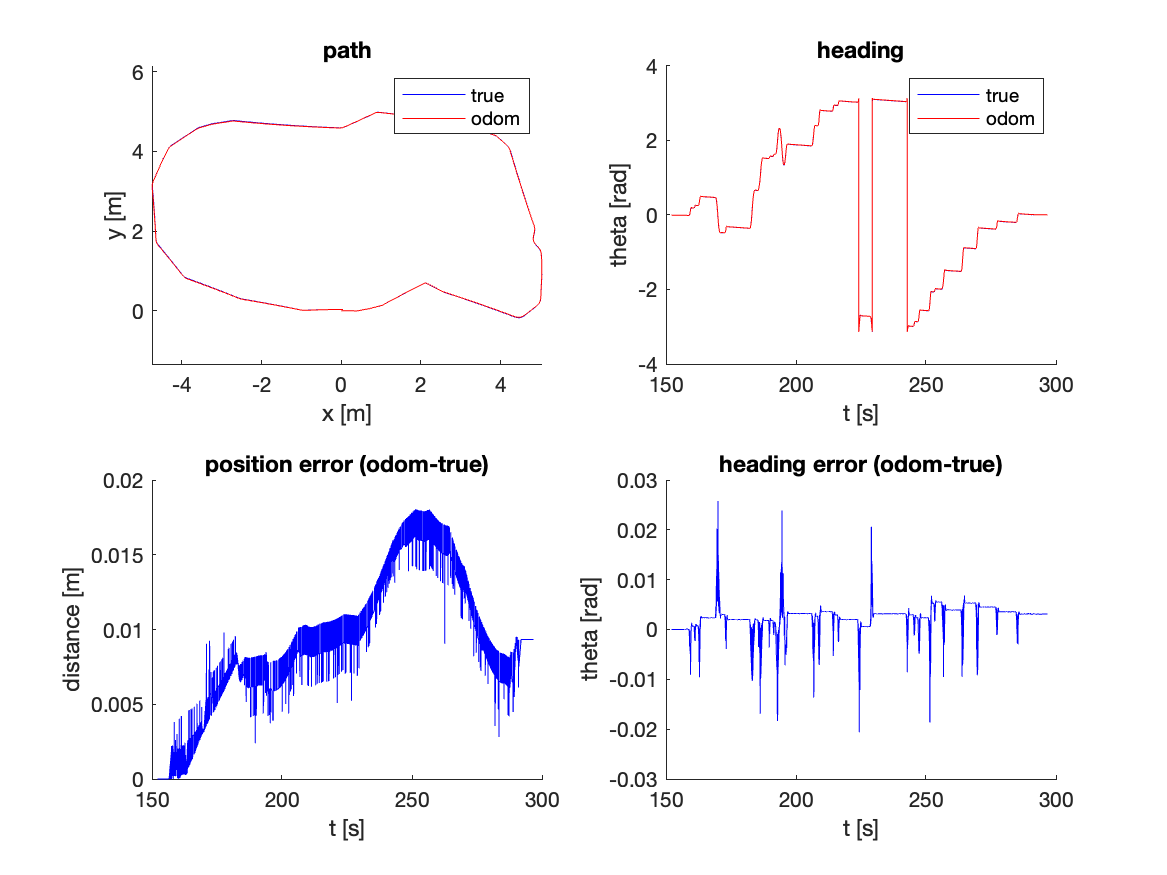
\includegraphics[width=0.8\textwidth]{ass1_q1.png}
    \caption{Noise-free wheel odometry robot pose estimates and error}
\end{figure}

\section{Question 2}
This question introduced gaussian noise to the wheel odometry measurements, which was then used to estimate the robot's pose over time.
The purpose of this question was to demonstrate the degradation of the pose estimate accuracy when using the algorithm from Question 1 with noisy sensor readings.
\textbf{Figure 2} shows the estimated robot pose path over time with noisy wheel odometry measurements for 100 random trials in red, and the ground truth robot pose in blue.
Comparing the performance of the algorithm to Question 1, it is clear that the pose estimate error is significantly higher when noise is introduced. While the general path
structure is still captured, detailed localization is missed, thus providing motivation for the mean and uncertainty pose estimate equations derived
in lecture.

\begin{figure}[h!]
    \centering
    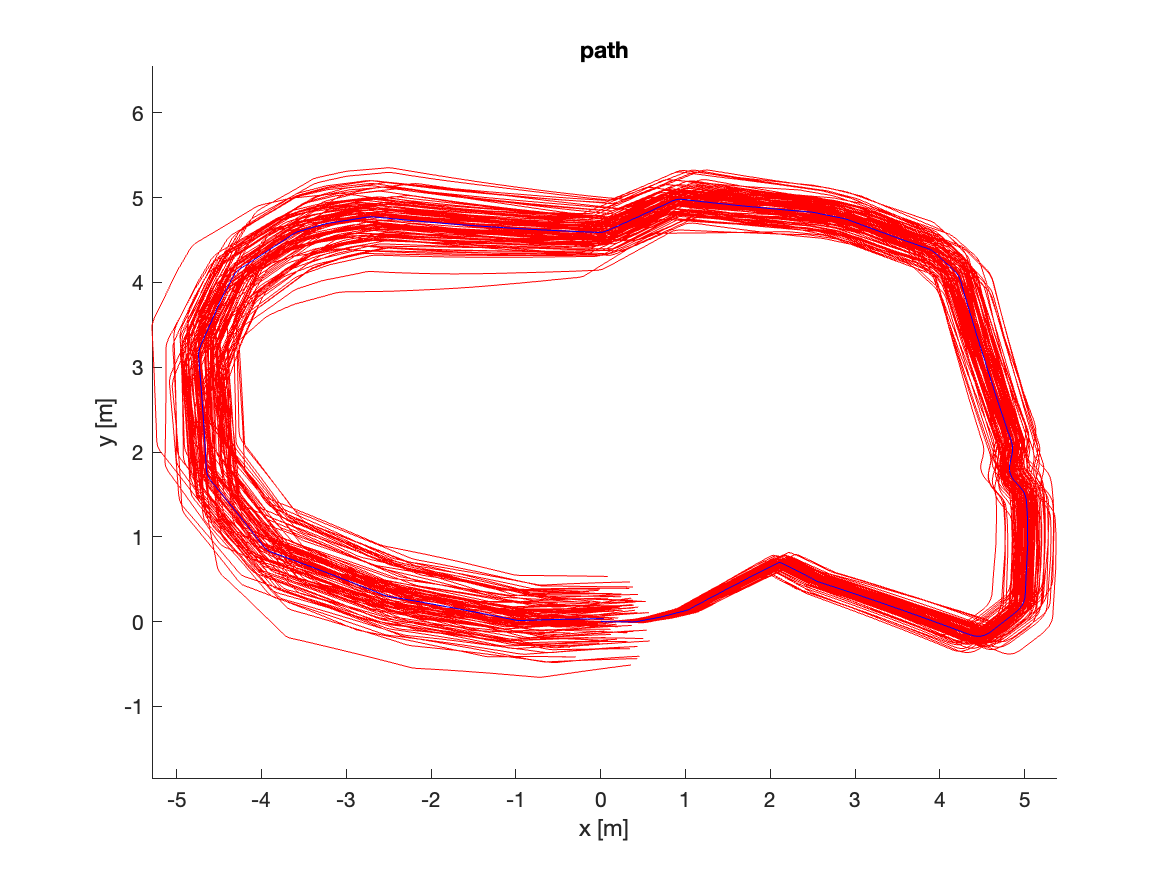
\includegraphics[width=0.8\textwidth]{ass1_q2.png}
    \caption{Comparison between noise-free and noisy wheel odometry robot pose estimates. The noisy wheel odometry robot pose estimates are shown in red, while the noise-free wheel odometry robot pose estimates are shown in blue.}
\end{figure}

\section{Question 3}
Question 3 extended the concepts of Question 2 by emphasizing the importance of considering sensor noise
when using the data to build maps. The noise-free and noisy wheel odometry measurements are
used with the LIDAR scan data to generate maps of the environment with respect to the initial robot pose.
To get the scan data in the initial frame, the data is first transformed to the current robot pose using the fact that origin of the laser scans is about 10 cm behind the origin of the robot.
Using the transformed $x$ and $y$ components of the laser data, the current robot pose from the wheel odometry is used to generate a transformation
matrix to get the laser scan data with respect to the initial frame. More specifically, the current robot $\theta$ estimate is applied
to the laser scan data through an elementary rotation matrix about the $z$ axis. The estimated $x$ and $y$ components of the robot pose are then used to
translate the data to a position in the initial frame. The same process is done for the noise-free and noisy wheel odometry measurements, and the results are shown in \textbf{Figure 3}.
From the figure it is clear that the introduction of noise into the system significantly degrades the quality of the map generated. While the general structure of the map is still captured,
many details are positioned relatively far off from the ground truth map. Moreover, this demonstrates the importance of accounting for sensor noise when estimating the robot pose from
wheel odometry measurements, as stochastic model representations can greatly improve estimates and map generation capabilities.

\begin{figure}[h!]
    \centering
    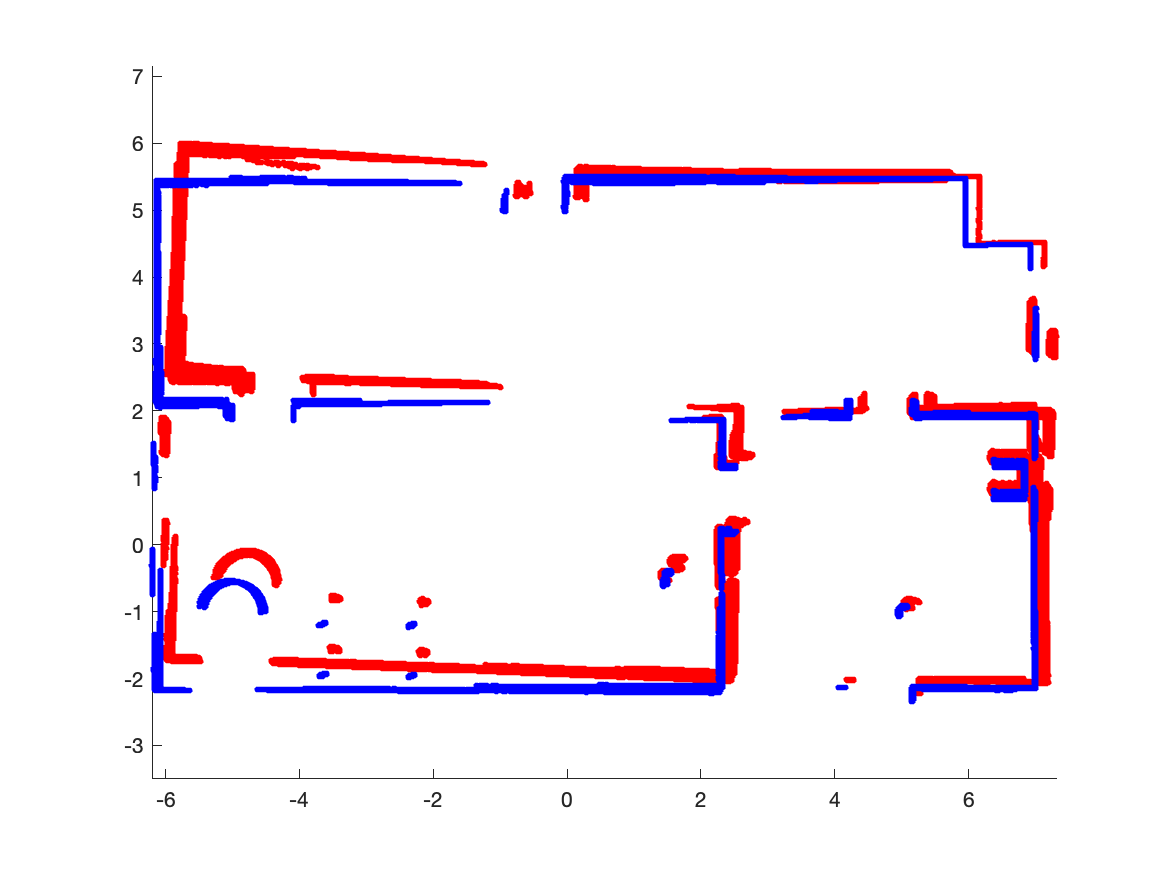
\includegraphics[width=1\textwidth]{ass1_q3.png}
    \caption{Map generation comparison between noise-free and noisy wheel odometry with respect to the initial robot pose. The noisy results are shown in red, while the noise-free results are shown in blue.}
\end{figure}

\section{MATLAB Code}

The MATLAB code for these implementations are provided here, as well as are attached in the submission.

\lstinputlisting[
frame=single,
numbers=left,
style=Matlab-editor
]{ROB521_assignment2.m}

\end{document}